%!TEX root = ../thesis.tex
\section{Client: Entwurf und Implementierung}

Bereits im Praxisprojekt \citep{Maemecke2017}, welches dieser Arbeit voran ging, wurde der komponentenbasierte Ansatz zur Programmierung von Browser-Frontends näher betrachtet. Eine Komponente ist ein modularer, in sich geschlossener Teil eines User Interfaces, der für \emph{eine} Aufgabe zuständig ist. Die Aufgabe einer Komponente kann nicht nur das Anzeigen von Daten oder anderer Elemente sein, sondern auch die Verwaltung von Daten und die Kommunikation mit einer API.

Mit diesem Ansatz lassen sich stabile, skalierbare und testbare Anwendungen für den Browser entwickeln.

Der komponentenbasierte Gedanke wird nicht nur bei der Programmierung, sondern auch bei der Gestaltung von \acp{UI} verfolgt. Design-Programme wie Sketch\footnote{https://www.sketchapp.com/} sind darauf ausgelegt, ein User Interface in Komponenten zu gestalten.

Dieses Kapitel beschäftigt sich mit der kompletten Entstehung des Clients: von der Planung über die Gestaltung bis hin zur Implementierung.

\subsection{Aufbau des User Interfaces}
\label{subsec:entwurf-user-interface}

Das User Interface der Webanwendung besteht aus verschiedenen \emph{Screens}. Ein Screen lässt sich umgangssprachlich als ``Unterseite'' beschreiben. Für den Nutzer sind vor allem drei Screens wichtig:

\begin{itemize}
  \item Chronologische Auflistung aller Build-Prozesse (Historie)
  \item Übersicht des letzten Build-Prozesses je Pipeline (neueste Build-Prozesse)
  \item Einzelansicht eines Build-Prozesses (Detail)
\end{itemize}

Screens mit Formularen, beispielsweise zum Erstellen einer Pipeline, wurden außen vor gelassen.

\subsubsection{Content Inventory}

Ein \emph{Content Inventory}\footnote{vgl. https://github.com/north/north\#content-inventory, abgerufen am 23.10.2017} ist eine Auflistung aller verfügbarer Daten, welches beim De\-sign\-pro\-zess dabei hilft, einen Überblick über alle verwendbaren Daten zu behalten und Prioritäten herauszuarbeiten.

In \tabref{tab:content-inventory} ist das Content Inventory auf die wichtigsten anzuzeigenden Komponenten bzw. Entitäten aufgeteilt.

\begin{table}[H]
  \scriptsize
  \begin{tabularx}{\textwidth}{| l | p{4cm} | l | X |}
    \hline
    \textbf{Objekt} & \textbf{Attribut} & \textbf{Typ} & \textbf{Notiz} \\ \hline
    \multirow{2}{*}{Projekt} & Titel & text &  \\ \cline{2-4}
      & Git URL & text & Nicht zwingend anzuzeigen \\ \hline
    \multirow{3}{*}{Pipeline} & Titel & text &  \\ \cline{2-4}
      & Bezeichner & text & Für Zuordnung in .warp.yml \\ \cline{2-4}
      & Regex-Auslöser & text &   \\ \hline
    \multirow{13}{*}{Build-Prozess} & Titel & text & Titel der Pipeline \\ \cline{2-4}
      & Nummer & integer &  \\ \cline{2-4}
      & Status & enum & queued, init, active, success, failed, stopped \\ \cline{2-4}
      & Startzeit & datetime &  \\ \cline{2-4}
      & Endzeit & datetime & bei aktivem Prozess nicht vorhanden \\ \cline{2-4}
      & Dauer & time & Ergibt sich aus Start- und Endzeit \\ \cline{2-4}
      & Durchschnittliche Dauer & time &  \\ \cline{2-4}
      & Differenz: Dauer und Durchschnittliche Dauer & time &  \\ \cline{2-4}
      & Git Reference & text & Branch oder Tag \\ \cline{2-4}
      & Commit SHA & text &  \\ \cline{2-4}
      & Commit Nachricht & long text & Kann mehrere Zeilen lang sein, sollte gekürzt werden \\ \cline{2-4}
      & User Bild & image & quadratisch \\ \cline{2-4}
      & User Name & text &  \\ \hline
    \multirow{5}{*}{Stage} & Titel & text &  \\ \cline{2-4}
      & Nummer & integer & Fortlaufende Nummerierung der Stages \\ \cline{2-4}
      & Status & enum & queued, init, active, success, failed, stopped \\ \cline{2-4}
      & Startzeit & datetime &  \\ \cline{2-4}
      & Endzeit & datetime & bei aktiver Stage nicht vorhanden \\ \cline{2-4}
      & Dauer & time & Ergibt sich aus Start- und Endzeit \\ \hline
    \multirow{5}{*}{Step} & Titel & text &  \\ \cline{2-4}
      & Befehl & text &  \\ \cline{2-4}
      & Status & enum & queued, init, active, success, failed, stopped \\ \cline{2-4}
      & Startzeit & datetime &  \\ \cline{2-4}
      & Endzeit & datetime & bei aktiver Stage nicht vorhanden \\ \cline{2-4}
      & Dauer & time & Ergibt sich aus Start- und Endzeit \\ \cline{2-4}
      & Ausgabe & long text & kann sehr lang werden \\ \hline
  \end{tabularx}
  \caption{Content Inventory}
  \label{tab:content-inventory}
\end{table}

\subsection{Visualisierung der Build-Historie}
\label{subsec:visualisierung-build-history}

Die Historie ist eine chronologische Auflistung aller Builds des Projekts. Aus ihr wird schnell ersichtlich, wann es zu Fehlern kam und wann diese behoben wurden. Viele Details zum einzelnen Build-Prozess sind daher nicht notwendig.

\begin{figure}[h]
  \caption{Kompakte Build-Prozess Komponenten mit positivem und negativem Status}
  \label{fig:build-process-short}
  \centering
    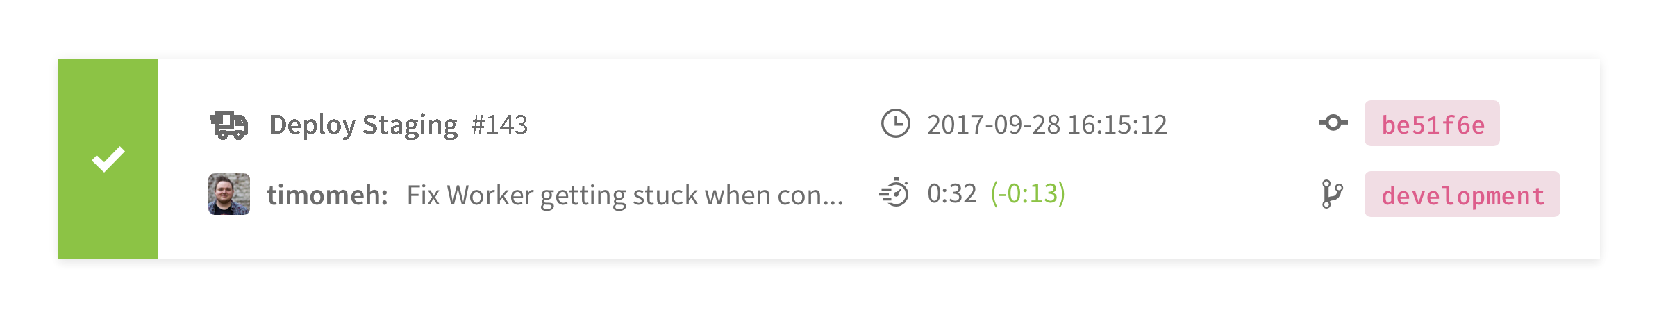
\includegraphics[width=\textwidth]{assets/build-overview-finished}
    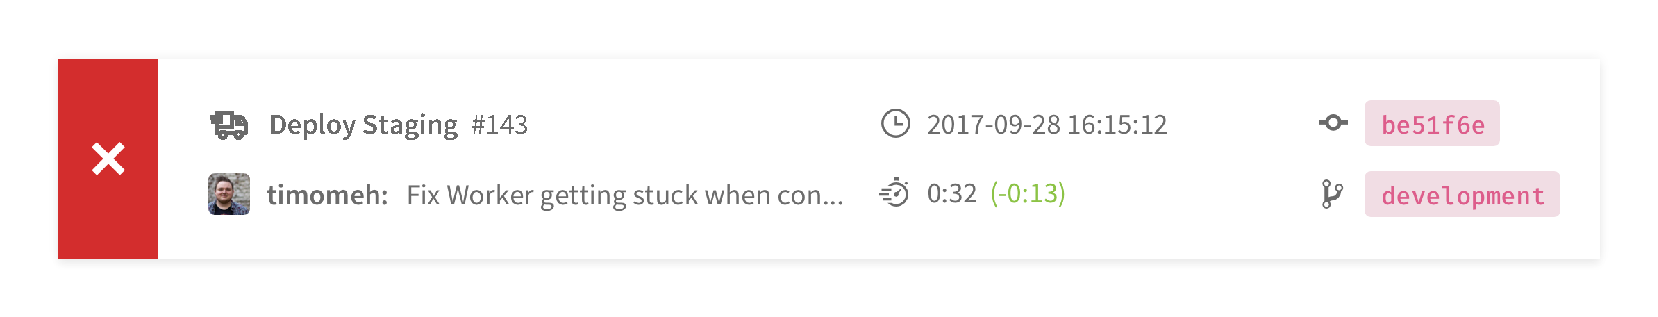
\includegraphics[width=\textwidth]{assets/build-overview-failed}
\end{figure}

Zu den wichtigsten Informationen eines Build-Prozesses gehört sein Status. Daher ist der Status in der Komponente aus \figref{fig:build-process-short} gut sichtbar links platziert. Weitere Daten in dieser Komponente wurden auf die wichtigsten Informationen reduziert.

Die Informationen wurden auf feste vertikale Ebenen aufgeteilt. Bei der Auflistung entsteht dadurch ein einheitliches Bild ohne visuelle Störungen.

Die Komponente ist nicht sehr hoch, damit mehr Elemente gleichzeitig im Viewport sichtbar sind (siehe \figref{fig:build-history}).

\begin{figure}[H]
  \caption{Chronologische Auflistung der Build-Prozesse}
  \label{fig:build-history}
  \centering
    \includegraphics[width=\textwidth]{assets/build-history}
\end{figure}

\subsection{Visualisierung der neuesten Build-Prozesse}

Eine der wichtigsten Informationen sind die neusten Builds. Zu jeder Pipeline wird der aktuellste Build-Prozess angezeigt. Daraus wird direkt ersichtlich, ob es aktuell Probleme gibt, und welche Version der Software auf welche Umgebung deployed wurde.

Hierfür wird im Vergleich zur Historie (siehe \fullref{subsec:visualisierung-build-history}) eine Komponente mit mehr Informationen benötigt.

\begin{figure}[h]
  \caption{Informationsreiche Build-Prozess Komponenten mit positivem Status}
  \label{fig:build-process-detail}
  \centering
    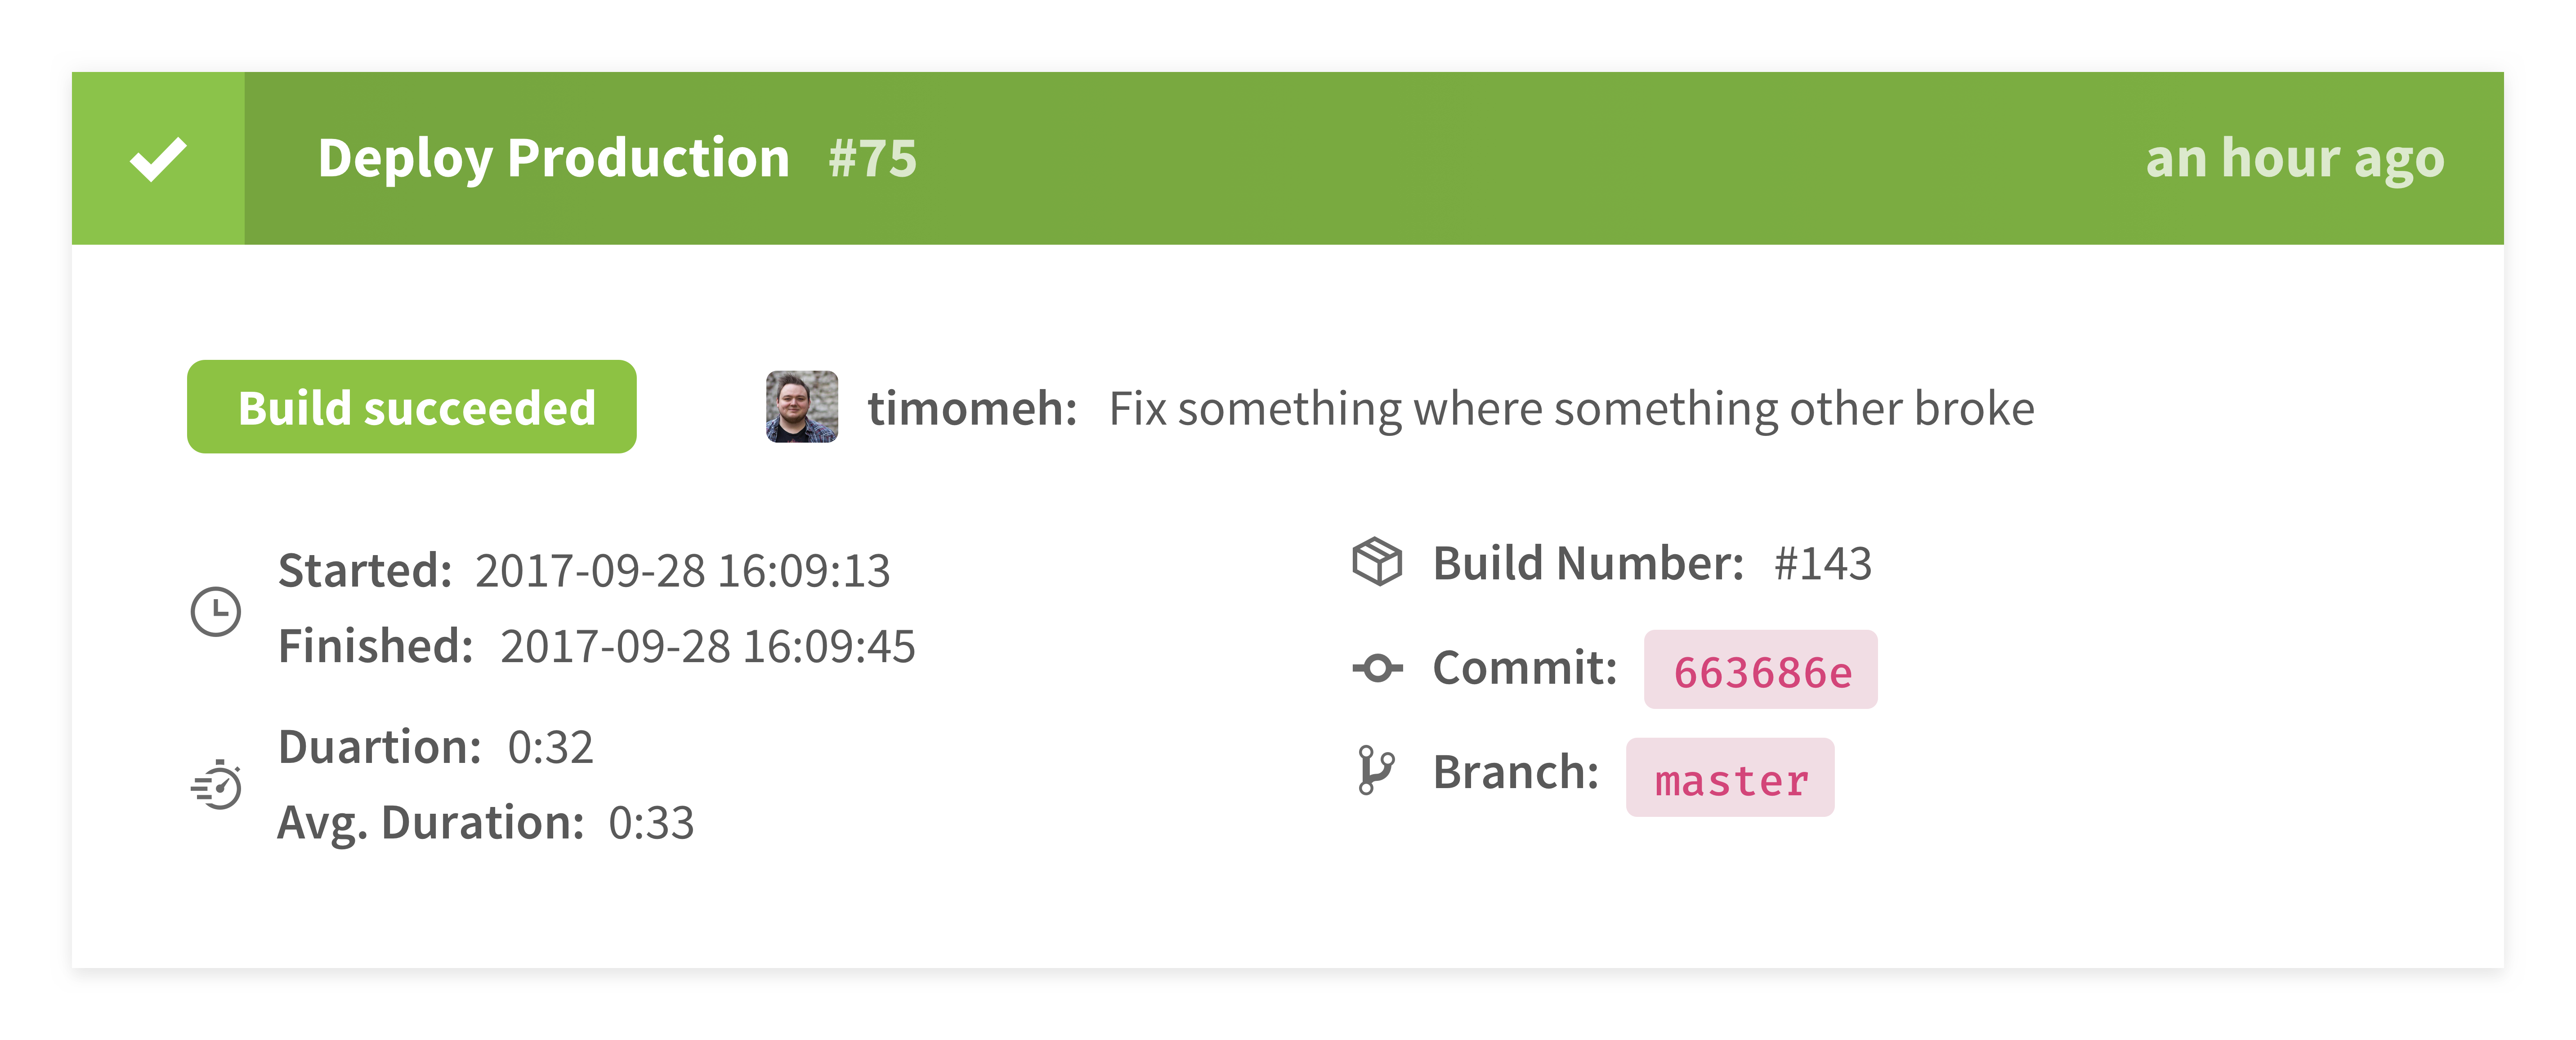
\includegraphics[width=\textwidth]{assets/build-detail-finished}
\end{figure}

Die Komponente in \figref{fig:build-process-detail} ist im Vergleich zur kleineren Komponente in \figref{fig:build-process-short} anders strukturiert, da der Fokus nicht mehr auf der Auflistung sondern dem einzelnen Build-Prozess liegt. Trotzdem enthält sie visuelle Ähnlichkeiten, damit ein Bezug zwischen beiden Komponenten erkennbar bleibt.

Die Informationen des Build-Prozesses besitzen neben einem passenden Icon nun auch eine textuelle Bezeichnung, um Verwirrung durch die Masse an Daten zu vermeiden.

Bei einem aktiven Build-Prozess ist an dieser Stelle eine Fortschrittsanzeige sinnvoll. Manche Anwendungen (wie Jenkins, siehe \fullref{sec:analyse-jenkins}) verwenden hierfür einen Ladebalken mit prozentualem Fortschritt. Diese Anzeige ist jedoch irreführend: Nachdem ein Schritt in einem Build-Prozess gestartet wurde, kennt die Anwendung nicht den Fortschritt innerhalb des Schrittes. Sie weiß nur, ob der Befehl gestartet und ob er beendet wurde. Die Anwendung weiß auch nicht, wie lange ein Schritt dauert\footnote{Die Dauer eines Schrittes ließe sich schätzen, indem ein Durchschnittswert aus früheren Build-Prozessen errechnet wird.}. Möglicherweise dauert ein bestimmter Schritt um ein vielfaches länger als andere Schritte.

\begin{figure}[h]
  \caption{Informationsreiche Build-Prozess Komponenten mit aktivem Status}
  \label{fig:build-process-detail-active}
  \centering
    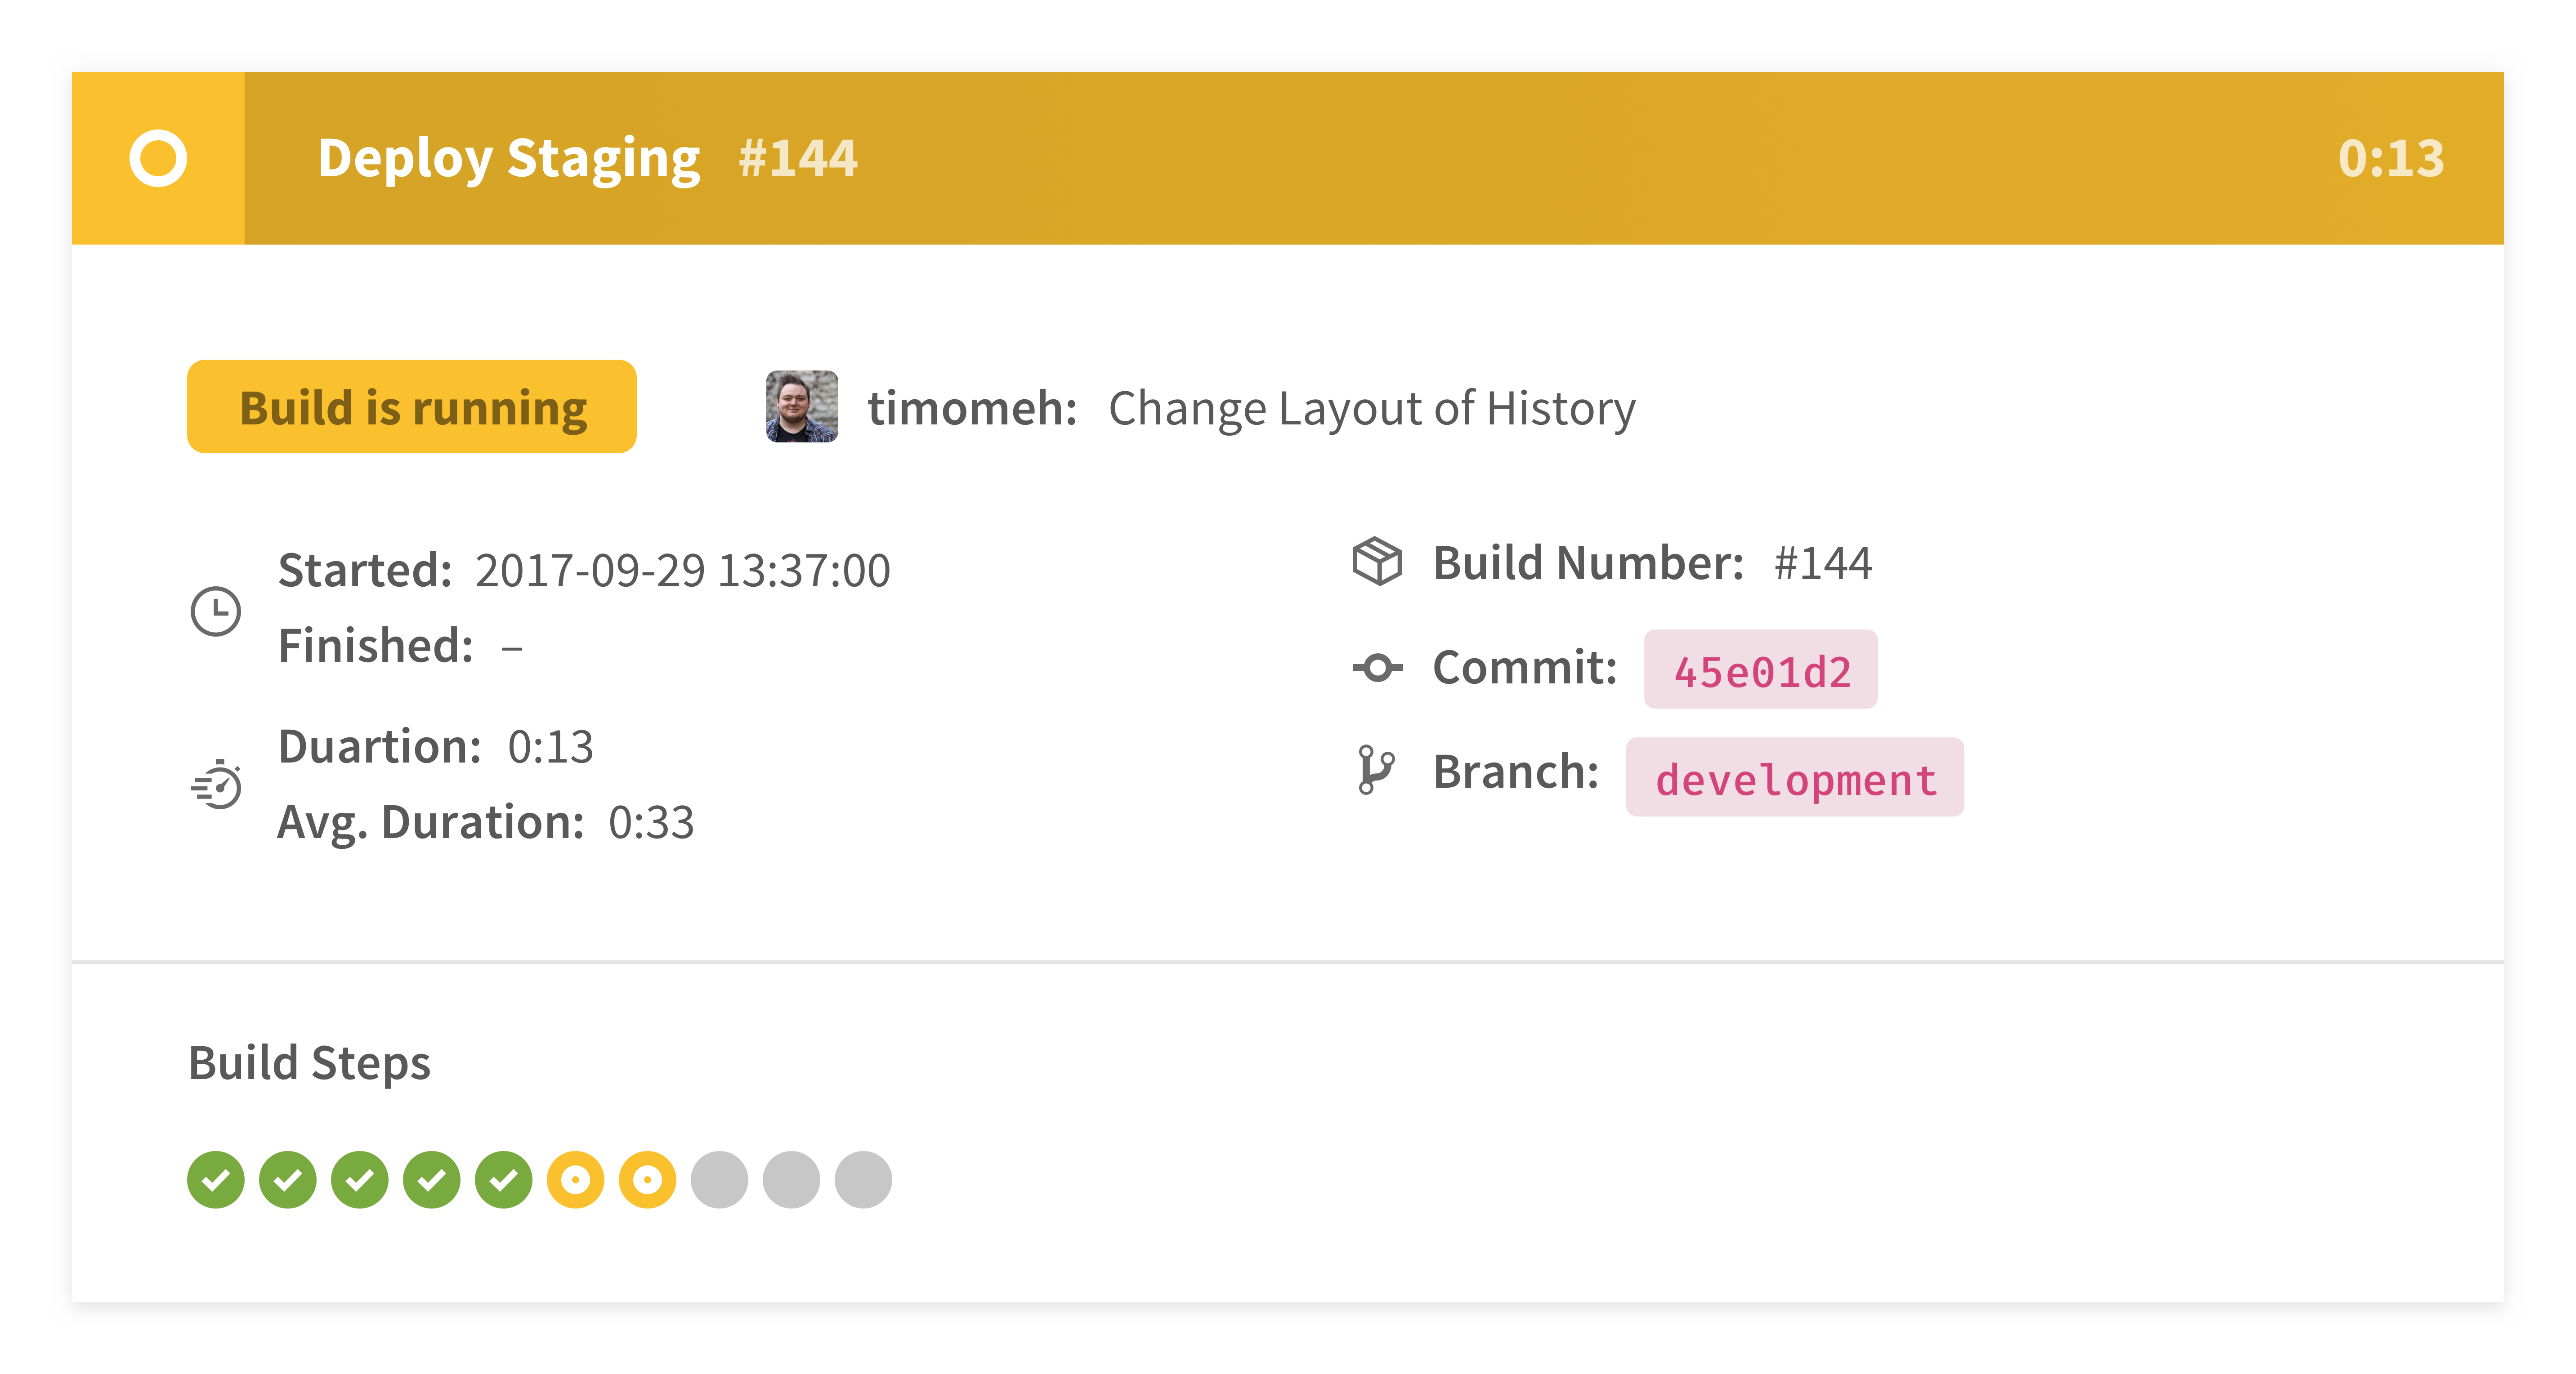
\includegraphics[width=\textwidth]{assets/build-detail-active}
\end{figure}

Daher werden die Schritte auch als solches in vereinfachter Darstellung aufgelistet, wie in \figref{fig:build-process-detail-active} zu sehen. Der Nutzer sieht, aus wie vielen Schritten ein Build-Prozess besteht, wie viele davon beendet wurden und wie viele noch ausstehen.

Auf dem Screen (siehe \figref{fig:latest-builds}) sind diese Komponenten nach absteigendem Datum sortiert. Ein größerer Abstand und die auffälligen durchgezogenen Farbbalken helfen bei der visuellen Trennung der Komponenten voneinander, damit der Fokus auf der einzelne Komponente bleibt.

\begin{figure}[H]
  \caption{Übersicht der neuesten Build-Prozesse}
  \label{fig:latest-builds}
  \centering
    \includegraphics[width=\textwidth]{assets/latest-builds}
\end{figure}

\subsection{Visualisierung der Pipeline}

Die Visualisierung der gesamten Pipeline (also aller Stages und die Abfolge ihrer Schritte) ist für den Nutzer vor allem dann wichtig, wenn ein Build-Prozess fehlgeschlagen ist. Bei Erfolg des Prozesses wird die Detail-Ansicht eher nicht benötigt.

In der Detail-Ansicht lässt sich erkennen, an welcher Stelle der Build-Prozess fehlgeschlagen ist und was die Ausgabe des fehlgeschlagenen Befehls war.

Die Stärke der Anwendung, dass Schritte beliebig tief in Gruppen verschachtelt werden können, ist gleichzeitig eine Schwäche bei der Visualisierung. Die Pipeline soll übersichtlich dargestellt werden, was sehr schwierig ist, wenn sich Schritte beliebig aufteilen können und parallele Prozesse entstehen. Zudem soll die Breite des Viewports nicht überschritten werden, wodurch der Nutzer horizontal und vertikal scrollen müsste.

Letztendlich wurde die Visualisierung in \figref{fig:pipeline-overview} gestaltet, bei der alle Schritte chronologisch untereinander aufgelistet werden, und parallele Prozesse nebeneinander angezeigt werden.

\begin{figure}[h]
  \caption{Einzelansicht des Build-Prozesses}
  \label{fig:pipeline-overview}
  \centering
    \includegraphics[width=\textwidth]{assets/pipeline-overview}
\end{figure}

Um keine weiteren visuelle Elemente einzuführen, wurden Designelemente der Historie (siehe \fullref{subsec:visualisierung-build-history}) wiederverwendet.

Ein Nachteil dieser Visualisierung ist, dass bei zu vielen parallelen Prozessen die einzelnen Schritte sehr schmal werden können. Eine Pipeline mit sehr vielen verschachtelten parallelen Prozessen kann allerdings auch ein Anzeichen für einen schlechten Aufbau der Pipeline sein.

\subsection{React und Redux}
\label{subsec:react-redux}

\textbf{React} ist eine Bibliothek für JavaScript, mit der sich komponentenbasierte User Interfaces für den Browser programmieren lassen. Wie schon im Praxisprojekt \citep{Maemecke2017} ausgearbeitet, eignet sich React besonders für dynamische Web\-anwendungen bzw. \acp{SPA} mit komplexen Funktionalitäten.

React wird von Facebook entwickelt und seit 2011 auf facebook.com verwendet. 2013 wurde React als Open Source Projekt veröffentlicht. Mittlerweile besitzt React eine sehr große und stetig wachsende Community, und wird auch von vielen Unternehmen und Projekten genutzt. Zu den Bekanntesten zählen u.a. Twitter, Netflix, Paypal, Reddit, Airbnb und viele mehr\footnote{vgl. https://github.com/facebook/react/wiki/sites-using-react. Tatsächlich ist die Verwendung von React aktuell so weit verbreitet, dass eine komplette Auflistung nur der bekanntesten Unternehmen schon den Rahmen sprengen würde.}.

\emph{Ein} Konzept in React ist der \emph{State}. In ihm werden Daten gespeichert, die zur Anzeige des aktuellen Zustands einer Komponente benötigt werden. Jede Komponente kann ihren eigenen State verwalten. \citep[State and Lifecycle]{ReactDocs}

Bei großen Anwendungen mit vielen Daten, die in verschiedenen Komponenten benötigt werden, wird die State-Verwaltung in voneinander getrennten Komponenten schnell schwierig. Zur Lösung dieses Problems gibt es die JavaScript-Bibliothek \textbf{Redux}.

Mit Redux lässt sich ein globaler State verwalten, auf den alle Komponenten zugreifen können. Wenn eine Komponente Daten im globalen State modifiziert, werden die Änderungen daran direkt in allen anderen Komponenten bekannt, die auf diese Daten zugreifen.

\subsection{Komposition als An\-wen\-dungs\-struk\-tur}
\label{subsec:komposition}

Komposition ist eins der Hauptmerkmale von Komponenten. Komposition bedeutet, dass durch das Zusammenspiel von mehreren Komponenten eine größere Aufgabe erfüllt wird. Jede Komponente ist dabei für einen Teil der Aufgabe zuständig. \citep[Kapitel 1]{Maemecke2017}

Man kann Komposition auch zur Modellierung von Daten-Abhängigkeiten nutzen: eine Komponente (A) ruft asynchron Daten von der \ac{API} auf. Während die Daten geladen werden, kann in Komponente A ein Ladeindikator angezeigt werden. Wenn die Daten geladen wurden, kann Komponente A eine weitere Komponente (B) anzeigen, welche die geladenen Daten darstellt.

Komponente B kann sich somit rein um die Darstellung der Daten kümmern. Zu keinem Zeitpunkt benötigt Komponente B eine Abfrage, ob die Daten bereits vorhanden sind.

Die Komposition von Abhängigkeiten kann tiefer verschachtelt werden. Im gerade genannten Beispiel kann Komponente B wiederum weitere Daten laden, die auf den Daten von Komponente A aufbauen.

In der Anwendung wird diese Art der Komposition als Grundgerüst der Anwendungsstruktur verwendet. \figref{fig:komposition} zeigt außerdem, was nach einer Interaktion des Nutzers geschieht. Beim initialen Aufruf der Anwendung wird die komplette Anwendungsstruktur für diesen Screens generiert. Wenn der Nutzer auf einen anderen Screen navigiert, wird nur die Komponente mit den alten Daten durch eine neue Komponente ausgetauscht.

\begin{figure}[h]
  \caption{Komposition von Komponenten als Anwendungsstruktur}
  \label{fig:komposition}
  \centering
    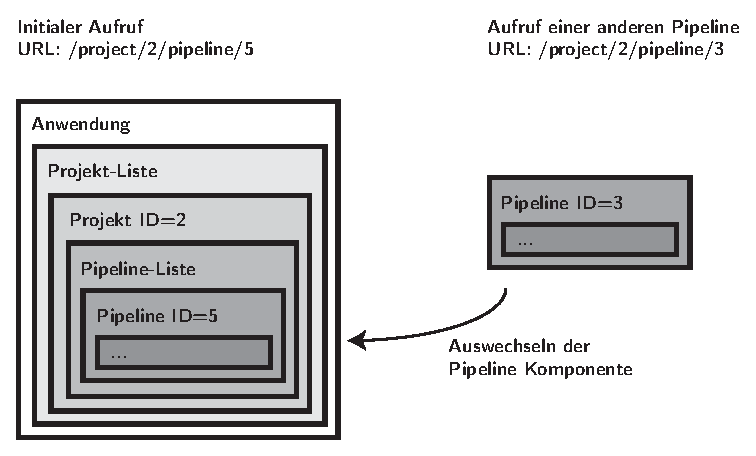
\includegraphics[width=\textwidth]{assets/komposition}
\end{figure}

\subsection{Implementierung der Anwendungsstruktur}
\label{subsec:implementierung-struktur}

Zum asynchronen Laden der Daten wird der \emph{Lifecycle} einer Komponente genutzt.

Eine Komponente besitzt verschiedene Methoden, die in ihrem Lebenszyklus an bestimmten Stellen aufgerufen werden. Wird beispielsweise eine Komponente angezeigt (``mount''), wird direkt davor die Methode \texttt{componentWillMount()} aufgerufen, und direkt nachdem sie angezeigt wurde, wird \texttt{componentDidMount()} aufgerufen. Genauso wird die Methode \texttt{componentWillUnmount()} aufgerufen, sobald eine Komponente nicht mehr angezeigt wird. \citep[State and Lifecycle]{ReactDocs}

Wir nutzen die Lifecycle-Methode \texttt{componentWillMount()} um die Anfrage an die API zu starten, wie in \lstref{lst:project-will-mount} zu sehen.

\lstinputlisting
  [caption={ProjectContainer.js: Laden eines Projekts},
  label={lst:project-will-mount},
  firstline=1,
  lastline=5,
  language=js]
  {snippets/project-container.js}

\texttt{dispatch()} in Zeile 4 ist eine Method aus Redux. Durch sie werden Änderungen an den globalen State übermittelt. Die Methode \texttt{fetchProject()} startet eine Anfrage an die API mit der entsprechenden Projekt-ID. (Mehr dazu in \fullref{subsec:datenfluss-redux}.)

Im globalen State wird das Feld \texttt{project.isFetching} während der Anfrage auf \texttt{true} gesetzt. Sind die Daten angekommen, wird es auf \texttt{false} gesetzt. Damit kann entweder ein Ladeindikator angezeigt werden, oder die verschachtelte Komponente aufgerufen werden (siehe \lstref{lst:project-render}).

\lstinputlisting
  [caption={ProjectContainer.js: render-Methode},
  label={lst:project-render},
  firstline=7,
  lastline=23,
  language=js]
  {snippets/project-container.js}

Als verschachtelte Komponente kann \texttt{<Project />} dem gleichen Schema folgen. Sie würde dann dementsprechend nicht das Projekt abrufen (worum sich bereits der ProjectContainer gekümmert hat), sondern stattdessen eine Liste der Pipelines oder letzten Builds. Im nächsten \fullref{subsec:react-routes} wird eine Besonderheit dieser Komponente behandelt.

\subsection{Implementierung der Frontend-Routen}
\label{subsec:react-routes}

Die Komponente \texttt{Project} soll verschiedene Screens anzeigen (vgl. Auflistung in \fullref{subsec:entwurf-user-interface}). Je nach \acs{URL} wird die Historie, die neuesten Build-Prozesse oder die Details zu einem Build-Prozess angezeigt.

Bei der Implementierung dafür hilft die Bibliothek react-router\footnote{https://reacttraining.com/react-router/}. Mit ihr lassen sich Routen und die zugehörige Komponente definieren.

\lstinputlisting
  [caption={Project.js: Definition von Routen mit react-router},
  label={lst:project-routes},
  language=js]
  {snippets/project.js}

Die in \lstref{lst:project-routes} verlinkten Komponenten \texttt{BuildDetails}, \texttt{History} und \texttt{Latest\-Builds} folgen jeweils wieder dem in \fullref{subsec:implementierung-struktur} beschriebenen Aufbau. Daher benötigt die Komponente \texttt{Project} keinen API-Aufruf in einer Lifecycle-Methode. Der Aufruf wird an die zutreffende Komponenten ausgelagert.

\subsection{Asynchroner Datenfluss mit Redux}
\label{subsec:datenfluss-redux}

Zur Implementierung des Redux Stores gibt es eine Best Practice für asynchrone Redux-Actions\footnote{Siehe http://redux.js.org/docs/advanced/AsyncActions.html, abgerufen am 23.10.2017}. Zusammen mit der Bibliothek redux-thunk\footnote{Siehe https://github.com/gaearon/redux-thunk} können in einem \emph{Action Creator} weitere Actions und asynchrone Funktionen aufgerufen werden.

Eine Funktion wie beispielsweise \texttt{fetchProject()} aus \fullref{subsec:implementierung-struktur} besteht aus mehreren Aufrufen:

\begin{enumerate}
 \item Feld \texttt{isFetching} setzen
 \item API asynchron aufrufen
 \item Daten dem Store hinzufügen
 \item Feld \texttt{isFetching} entfernen
\end{enumerate}

Dieser Ablauf ist im Action Creator aus \lstref{lst:project-async-action} auch so implementiert.

\lstinputlisting
  [caption={redux/project.js: Asynchrone Action},
  label={lst:project-async-action},
  firstline=35,
  lastline=44,
  language=js]
  {snippets/project-store.js}

Die beiden aufgerufenen Funktionen \texttt{requestProject()} und \texttt{receiveProject()} (siehe \lstref{lst:project-action-creators}) geben die Actions aus, auf die der Reducer aus \lstref{lst:project-reducer} reagiert und somit den globale State modifiziert.

\lstinputlisting
  [caption={redux/project.js: Action Creators},
  label={lst:project-action-creators},
  firstline=26,
  lastline=33,
  language=js]
  {snippets/project-store.js}

\lstinputlisting
  [caption={redux/project.js: Redux Reducer},
  label={lst:project-reducer},
  firstline=1,
  lastline=24,
  language=js]
  {snippets/project-store.js}

Der Quelltext aus diesen Beispielen ist eine vereinfachte Version der tat\-säch\-lich\-en Implementierung. Anstatt an dieser Stelle das Projekt zu speichern, wird dort nur die ID gespeichert und das dazugehörige Objekt in einem anderen Reducer gespeichert, in dem auch andere Entitäten gespeichert werden.


\subsection{Aktualisierung der Daten über einen Websocket}

Während eines Build-Prozesses werden aktualisierte Daten des Builds über einen Websocket an den Client übertragen. Dadurch kann der aktuelle Stand des Prozesses in nahezu Echtzeit aktualisiert werden.

Wie in \fullref{subsec:implementierung-worker} erläutert, werden diese Aktualisierungen in einem Kanal je Projekt gesendet. Die Komponente \texttt{Project\-Con\-tain\-er}, die in \fullref{subsec:implementierung-struktur} beschrieben wurde, eignet sich sehr gut, um sich mit diesem Kanal zu verbinden.

Die Komponente wird durch die Methoden in \lstref{lst:project-websocket} ergänzt.

\lstinputlisting
  [caption={ProjectContainer.js: Verbinden mit Websocket},
  label={lst:project-websocket},
  firstline=1,
  lastline=17,
  language=js]
  {snippets/project-container-ws.js}

Die darin aufgerufene Klasse \texttt{Socket} ist ein eigenes Modul, welches auf die Socket-Implementation aus der JavaScript-Bibliothek von Phoenix zugreift.

\lstinputlisting
  [caption={socket.js: Constructor},
  label={lst:socket-constructor},
  firstline=1,
  lastline=7,
  language=js]
  {snippets/socket.js}

Bei der Instanziierung wird die \texttt{dispatch} Methode aus Redux als Pa\-ra\-me\-ter über\-ge\-ben. Dadurch kann das Modul auf den Redux Store zugreifen und den globalen State modifizieren. Änderungen am globalen State werden direkt in allen Komponenten angezeigt, die diese Daten anzeigen.

\lstinputlisting
  [caption={socket.js: Verbinden mit dem Projekt-Kanal},
  label={lst:socket-join},
  firstline=9,
  lastline=30,
  language=js]
  {snippets/socket.js}

Nachdem sich erfolgreich mit dem Kanal verbunden wurde, empfängt das Modul die aktualisierten Daten in einem \emph{Event Listener}. In den übertragenen Daten des Events (\texttt{payload}) ist zusätzlich zu der Entität auch ein Name des Events vorhanden. Anhand dieses Namens kann die entsprechende Funktion aufgerufen werden, um beispielsweise die Attribute eines Builds zu aktualisieren.

Wenn der Nutzer auf ein anderes Projekt wechselt, wird die Lifecycle-Methode \texttt{componentWillUnmount()} aufgerufen (siehe \lstref{lst:project-websocket}) und die Verbindung zum Kanal getrennt (siehe \lstref{lst:socket-leave}).

\lstinputlisting
  [caption={socket.js: Trennung der Verbindung},
  label={lst:socket-leave},
  firstline=32,
  lastline=43,
  language=js]
  {snippets/socket.js}

Bei den Quelltexten handelt es sich um eine vereinfachte Version zur besseren Ver\-ständ\-lich\-keit. Die reale Implementation gestaltet sich etwas komplexer, besitzt jedoch den gleichen Aufbau.
